% Copyright (C) 2012 Davidlohr Bueso <dave@gnu.org>

% GPT STUFF
\section{GPT Support}
\begin{frame}\frametitle{What is GPT?}
  A standard developed by Intel in the late '90s for the layout of the partition table on a physical hard disk.\newline

  It overcomes major limitations of MBRs and today forms part of the \textbf{UEFI} standard.
\end{frame}

\subsection{Benefits of GPT}
\begin{frame}\frametitle{Benefits of GPT}
  So, what's the big deal about GPT?
  \begin{itemize}
  \item Forget extended or logical DOS-like partitions. GPT can handle at least 128 partitions.
  \item 64-bit sectors gives us $2^{64}$ available sectors, or 9.4 Zb partitions (with 512 bytes).
  \item 32-bit CRC checksums to ensure data integrity.
  \item Redundant data structures help protect against disk errors.
  \end{itemize}
\end{frame}

\subsection{Drawbacks of GPT}
\begin{frame}\frametitle{Drawbacks of GPT}
  \begin{columns}
    \begin{column}{.25\linewidth}
      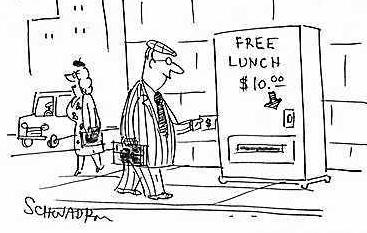
\includegraphics[scale=1.3]{img/freelunch}
    \end{column}
    \begin{column}{.7\linewidth}
      \begin{itemize}
      \item Compatibility
        \begin{itemize}
        \item OS
        \item Bootloaders
        \end{itemize}
      \item Non-standard schemes (Hybrid MBRs)
      \end{itemize}
    \end{column}
  \end{columns}
\end{frame}

\subsection{Fdisk and GPT}
\begin{frame}\frametitle{Fdisk \& GPT}
  \begin{itemize}
  \item Well known fact that fdisk didn't play well with GPT
    \begin{itemize}
      \item disklabel detection \emph{only}
      \item sends users to other tools (GNU parted)
      \item deals only with legacy DOS partitions.
    \end{itemize}
  \item Sept. 2012 we got full GPT support merged in mainline fdisk.
  \end{itemize}
\end{frame}

\subsection{Implementation Details}
\begin{frame}\frametitle{Some GPT Implementation Details}
  \begin{itemize}
  \item Deals with both legacy protective and hybrid MBRs.
  \item Updates checksums on the fly and not only when writing in-memory data to disk.
  \item Generous support for GUID partition types.
  \end{itemize}
\end{frame}
